\section{Refactoring} \label{sec:s4_refactoring}
%%% Intro paragraph --> Why do we refactor?

%%% How do we refactor?

%%% Summary --> Did the refactoring give us the desired results?

\subsection{Class Architecture}
In order to describe the structure design of the hotMap server, the UML v2.5 standard are used to express how the class hierarchy was designed. UML is a well known modeling language, for visualizing software system designs in order to more easily describe the static structure of a software system.
Therefore a UML class diagram are used for describing the model layer of the hotMap server.

Mixin is an language dependent functionality, which allows a class $A$ to contain methods from other classes or interfaces without having $A$ be a specialization of these other classes or traits. How class $A$ gain access to those methods through mixin are defined by the language. 

Scala does not have interfaces, but instead uses traits. These are similar but allow for default implementation of methods within the trait. When a concrete classes extends traits, it is called a realization of that trait, which in UML are indicated by a dashed arrow from the class to the interfaces. In scala traits can also be instantiated if all of its instance variables and methods have default implementions. In scala only traits can be mixed into classes or another trait.


In scala type aliases of mixin types are used to denoted a class or trait with a trait miexd into it. As an example of this we have on \cref{fig:class} that type $Point$ is a alias for any type which realizes the trait $Coordinate$ mixed with the trait $Weight$. UML cannot represent mixin, so it was chosen to show this by drawing a realization arrow with a mixin stereotype from the alias to the mixed type. Stereotypes are denoted by some text surrounded with $<<$ and $>>$ above the arrow.

\begin{sidewaysfigure}[htbp]
\centering
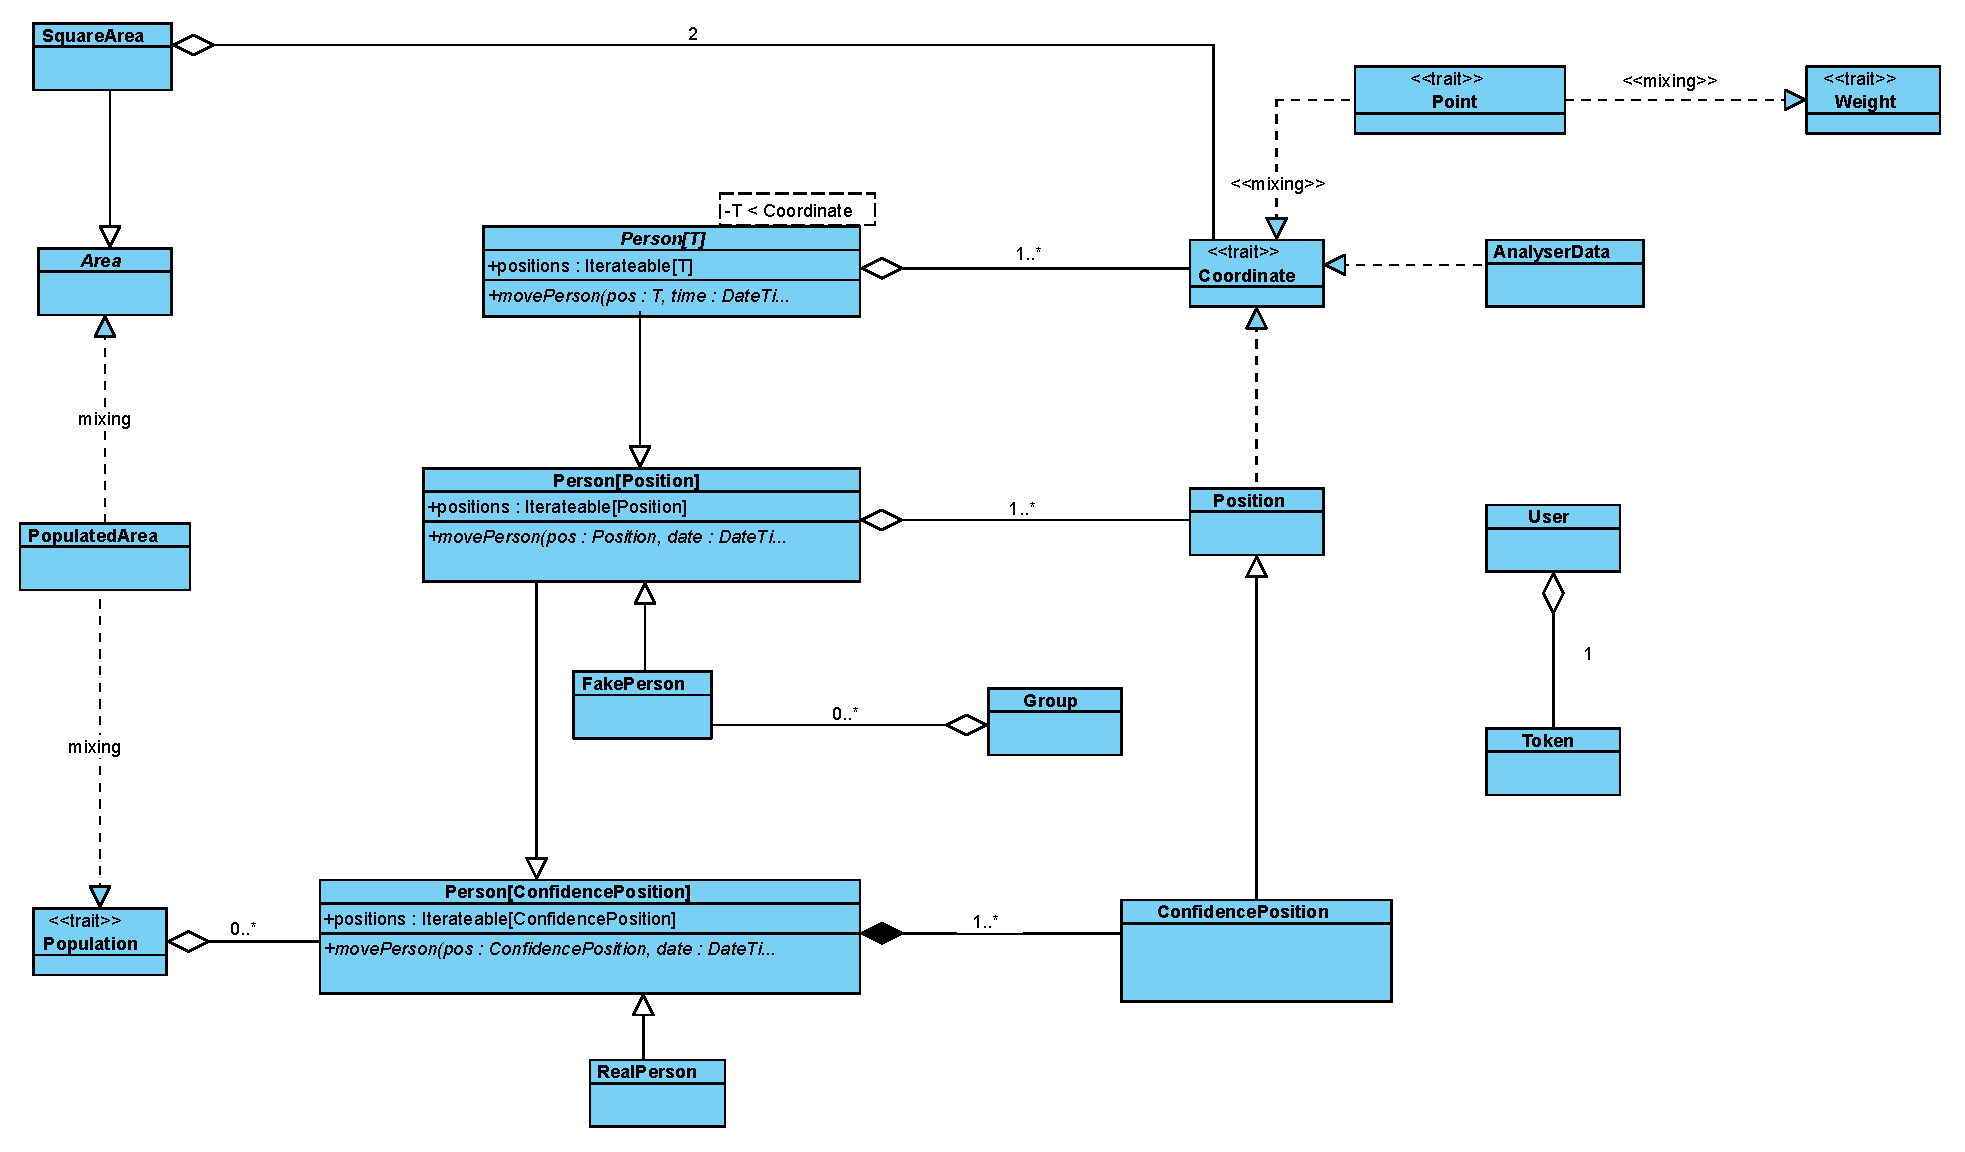
\includegraphics[width=\linewidth]{figures/class.eps}
\caption{Digraph.}
\label{fig:class}
\end{sidewaysfigure}


\subsection{Implementation of Asynchronous Analysis}
\label{sub:implementation_of_asynchronous_analysis}

As described in \cref{sub:Asynchronous_Analysis} the amount of calculations required can be reduced by analysing location data asynchronously from user requests, storing completed analyses. We assume that users will primarily monitor real-time crowd factors, therefore we will focus on optimising the real-time analysis.

This was implemented using a infinite loop running on another thread. This thread fetches and analyses position data from the aSTEP core. Completed analyses from this thread are stored in a global variable. When a user requests crowd factors the request handler will respond with data obtained from this global variable. 

There is one thread which writes data to the global variable, and potentially one thread per user reading data from this global variable. The global variable is a pointer to the result of the latest completed analysis. When the analysis of new data is completed, this pointer is changed atomically, in order to prevent race conditions. 

The infinite loop is repeated at most once per 5 seconds. In the case that an iteration of the loop takes longer than 5 seconds to complete, the next iteration will not start until the current iteration has completed. The 5 second limitation corresponds to the frequency at which the aSTEP core can supply updated data. One iteration of the loop consists of the following five stages: 

\begin{enumerate}
    \item \textbf{Process the position data:} At this stage all the fetched positions are associated with the corresponding person, based on a id received together with every position. This id identifies a single Wi-Fi device. Afterwards the method $movePerson$ is called for every instance of the class Person, with the corresponding new position as parameter, in order to add this position to a persons history.
    \item \textbf{Fetch position data:} This stage fetches position data from the aSTEP core.
    \item \textbf{Calculate analysis data:} The purpose of this stage is to calculate the list of $AnalyserData$ for each $Area$. This involves calculating all peoples heading direction and velocity, and encapsulate this in an instance of the class $AnalyserData$.
    \item \textbf{Analysis:} This stages analyses the data from the last stage, estimating the crowd factors of each $Area$.
    \item \textbf{JSON Conversion:} At the last stage the result of the analysis is converted into JSON format, which is then stored in the global variable used for user requests. 
\end{enumerate}

In summary, this implementation ensures that the data analysis is not performed for all users requesting real-time information, which improves the performance of the server. It also improves client side performance, as handling requests of analysed data takes less time. Another advantage of this implementation is that multiple users monitoring real-time crowd conditions will be shown the exact same information.
